%!TEX root = ../icassp2016.tex
\section{Experiments}
\label{sec:experiment}

\begin{table*}[ht!]
  \centering
\begin{tabular}{ llll }
    \toprule
    Method & Description & Signal Representation & Factorization Model \\
    \midrule
    CFM & Common Fate Model & STFT $\rightarrow$ Grid Slicing $\rightarrow$ 2D-DFT & $V(a,b,f,t) = P(a,b,f)\times H(t)$ \\
    NMF &\cite{virtanen2007monaural} w/o add.\ constraints & STFT & $V(f,t) = W(f)\times H(t)$ \\
    HR-NMF & High Resolution NMF model~\cite{magron15a} & Output of any filterbank (STFT, MDCT, \ldots)  & Subband AR filtering of NMF excitation \\
    MOD &\cite{barker13} using DFT filterbank& STFT $\rightarrow$ $|\ldots|$ $\rightarrow$ STFT along each bin & $V(f,m,t) = W(f)\times A(m)\times H(t)$ \\
    CFMM & Common Fate Magnitude Model & STFT $\rightarrow$ $|\ldots|$ $\rightarrow$ Grid Slicing $\rightarrow$ 2D-DFT & $V(a,b,f,t) = P(a,b,f)\cdot H(t)$ \\
    CFMMOD & CFMM with $a=1$ & STFT $\rightarrow$ $|\ldots|$ $\rightarrow$ Grid Slicing $\rightarrow$ 2D-DFT & $V(a,b,f,t) = P(a,b,f)\cdot H(t)$ \\
    \bottomrule
\end{tabular}
\caption{Overview of the evaluated algorithms}
\label{tab:methods}
\end{table*}

In this section, we present separation experiments utilizing CFM and we compare it with other methods.

\subsection{Synthetic Example}
\label{sub:Synthentic_Examples}

To illustrate the CFT representation we processed a mixture consisting of two sinusoidal sources. One source is a pure sine wave of fundamental frequency 440~Hz whereas the other is frequency modulated by a sinusoid of 6.3~Hz. In the first step an STFT with a DFT-length of 1024 samples and a hop-size of 256 samples was processed at a sample rate of 22.05~kHz. Patches of size $(N_a, N_b) = (32, 48)$ (not respecting overlaps) were then taken from the STFT output. Figure~\ref{fig:CFT} in Section~\ref{sub:CFT} then shows the Common Fate Transform for the mixture as described in Section~\ref{sec:model}. One can see that the CFT representation shows distinct patterns across time, suggesting that the factorization is able to separate the sources.

% \begin{figure}[b]
% \centering
% 		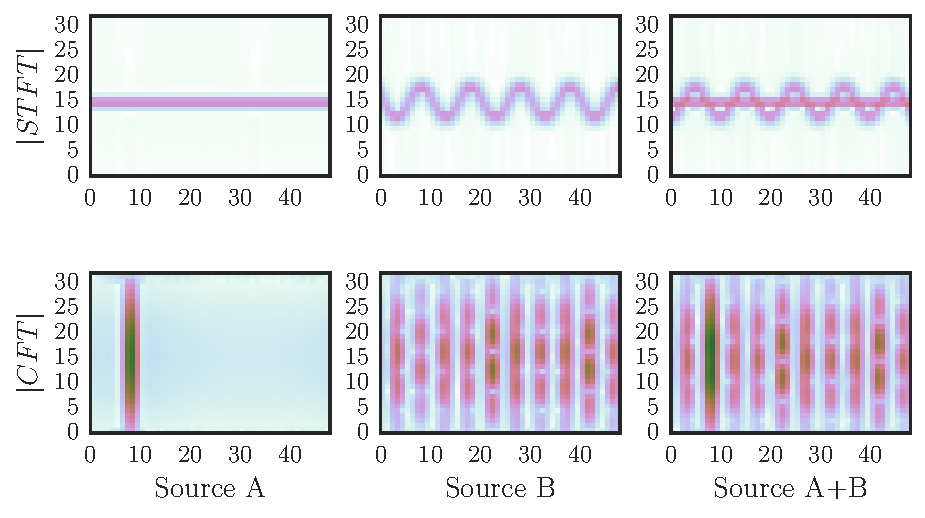
\includegraphics[width=0.95\columnwidth]{figures/gridplot.pdf}
% \caption{Examples of patches of size $(N_a, N_b) = (32, 48)$. The upper row shows magnitude values from the STFT output, the lower row the corresponding Common Fate Transform (CFT).}
% \label{fig:gridplot}
% \end{figure}

\subsection{Objective Evaluation on Unison Instrument Mixtures}

For an evaluation of the method, we selected five musical instruments' samples, all featuring vibrato: violin, cello, tenor sax, English horn, and flute. It is important to note that vibrato techniques differ between instruments: whereas the English horn and the flute only produce a very subtle modulation, the violin and tenor sax have powerful frequency modulations with a higher modulation frequency as well as a higher modulation index. The signals have each been generated by rendering C4 (261.63~Hz) notes in a state-of-the-art software sampler\footnote{\textsc{Vienna Symphonic Library} (\url{https://vsl.co.at})}. All samples last about three seconds. We then generated a combination of ten mixtures of two instruments each, each one generated with a simple SourceA --- SourceB --- (SourceA + SourceB) scheme. Data were encoded in 44.1 kHz / 16 bit.
For evaluation, we compared separation performance of six different methods, summarized in Table~\ref{tab:methods}:
\begin{description}[style=unboxed,leftmargin=0cm]
\item[CFM] For the CFM model, we took an STFT with frames of 1024 samples and a hop-size of 512 samples. The resulting complex spectrogram was then split into a grid of patches of size $(N_a, N_b) = (4, 64)$, each having a half-window overlap in both dimensions. For all experiments $\alpha$ and $\beta$ were set to 1.
\item[MOD] We implemented a modified version of~\cite{barker13} where for the sake of comparability, we used a STFT instead of a gammatone filterbank. A DFT length of 1024 and a hop-size of 512 samples were chosen. After taking the magnitude value, a second STFT of size 32 and hop-size 16 samples was computed for each frequency.
\item[CFMMOD] We selected patch sizes of $(N_a, N_b) = (1, 64)$ and modified the representation so that the magnitude spectrogram was used before computing the 2D-DFT.\@ This permits to compare the advantage of our proposed factorization model~(\ref{eq:NTF_model}) over MOD, when using the same kind of energy-modulation representation in both cases.
\item[CFMM] For comparing the influence of computing modulations over complex STFT or magnitude spectrograms, we tried our factorization model when the magnitude of the STFT is taken before 2D-DFT, with patches of the same size as for the CFM method.
\item[NMF] We took a standard NMF based method~\cite{virtanen2007monaural}. We highlight that taking a spectrogram with frames of length 1024 would not make a fair comparison, because the CFM model actually results in a larger frequency resolution. Therefore a comparable NMF is based on an STFT of DFT-length 32768.
\item[HR-NMF] See description in~\cite{magron15a}.
\end{description}
All factorizations ran for 100 iterations and were repeated five times. We chose $j=(2\ldots6)$ components for each factorization. For $j > 2$ we used oracle clustering to show the upper limit of SDR which can be achieved.

We ran the performance evaluation by using BSSeval~\cite{Vincentbsseval06}. The results of Signal to Distortion
Ratio (SDR), Signal to Interference Ratio (SIR), and Signal to Artifacts Ration (SAR) are depicted in Figure~\ref{fig:boxplot_overall}. Results indicate that the CFM model performs well in all measures. However, in terms of SIR the results of HR-NMF are better than CFM method. The results for CFMMOD indicate the positive influence of the CFM factorization compared to~\cite{barker13}.
The results of CFMM indicate that the complex CFT lead to better results. NMF did perform surprisingly well, which may only hold for our test set, where each source is active for a long period. This results in a cyclic stationary vibrato, revealing spectral side lobes at such a high resolution. With more than one component per source, the results of CFM do improve, but it can be seen that more than two components ($j=4$) will not increase the SDR values. The separation results and a full Python implementation of the CFM algorithm can be found on the companion website for this paper\footnote{\url{www.loria.fr/~aliutkus/cfm/}}.

% To understand the influence of the underlying matrix or tensor representation we additionally computed a normalized tensor correlation for each of the methods before before applying the factorization. Therefore for each source we compute the sum of the Hadamard product and normalize the output to the it's energy. The mean results of this correlation are shown in table~\ref{tab:correlation}.

\begin{figure}[ht!]
\centering
		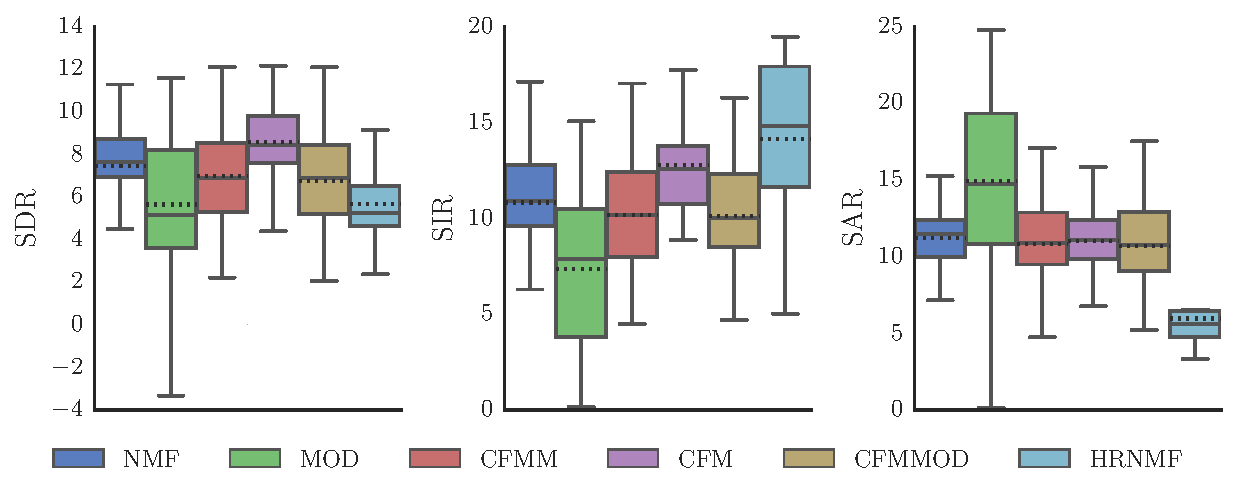
\includegraphics[width=0.90\columnwidth]{figures/boxplot.pdf}
\caption{Boxplots of BSS-Eval results of the unison dataset. Solid/dotted lines represent medians/means.}
\label{fig:boxplot_overall}
\end{figure}

\begin{figure}[ht!]
\centering
		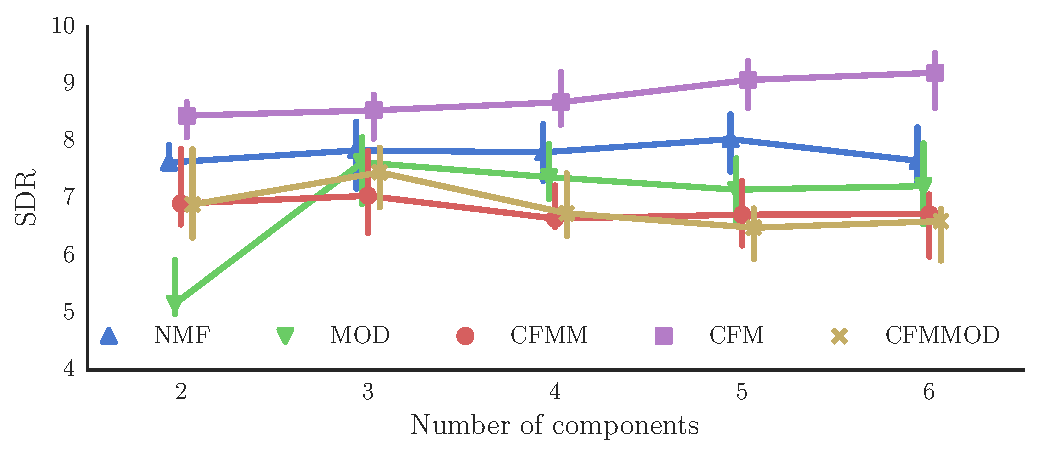
\includegraphics[width=0.90\columnwidth]{figures/iterations.pdf}
\caption{Boxplots of SDR values of the unison dataset over the number of components $j$. For $j>2$ oracle clustering was applied.}
\label{fig:iterations}
\end{figure}
